\begin{tikzpicture}
  \newlength{\unit}
  \setlength{\unit}{1.8cm}

  \tikzset{con/.style={-{Triangle[length=0.25cm, width=0.3cm]}, line width=0.1\unit}}

  \node[anchor=east, text width=1\unit, align=right] (source) at (0, 0) {%
    \tiny%
    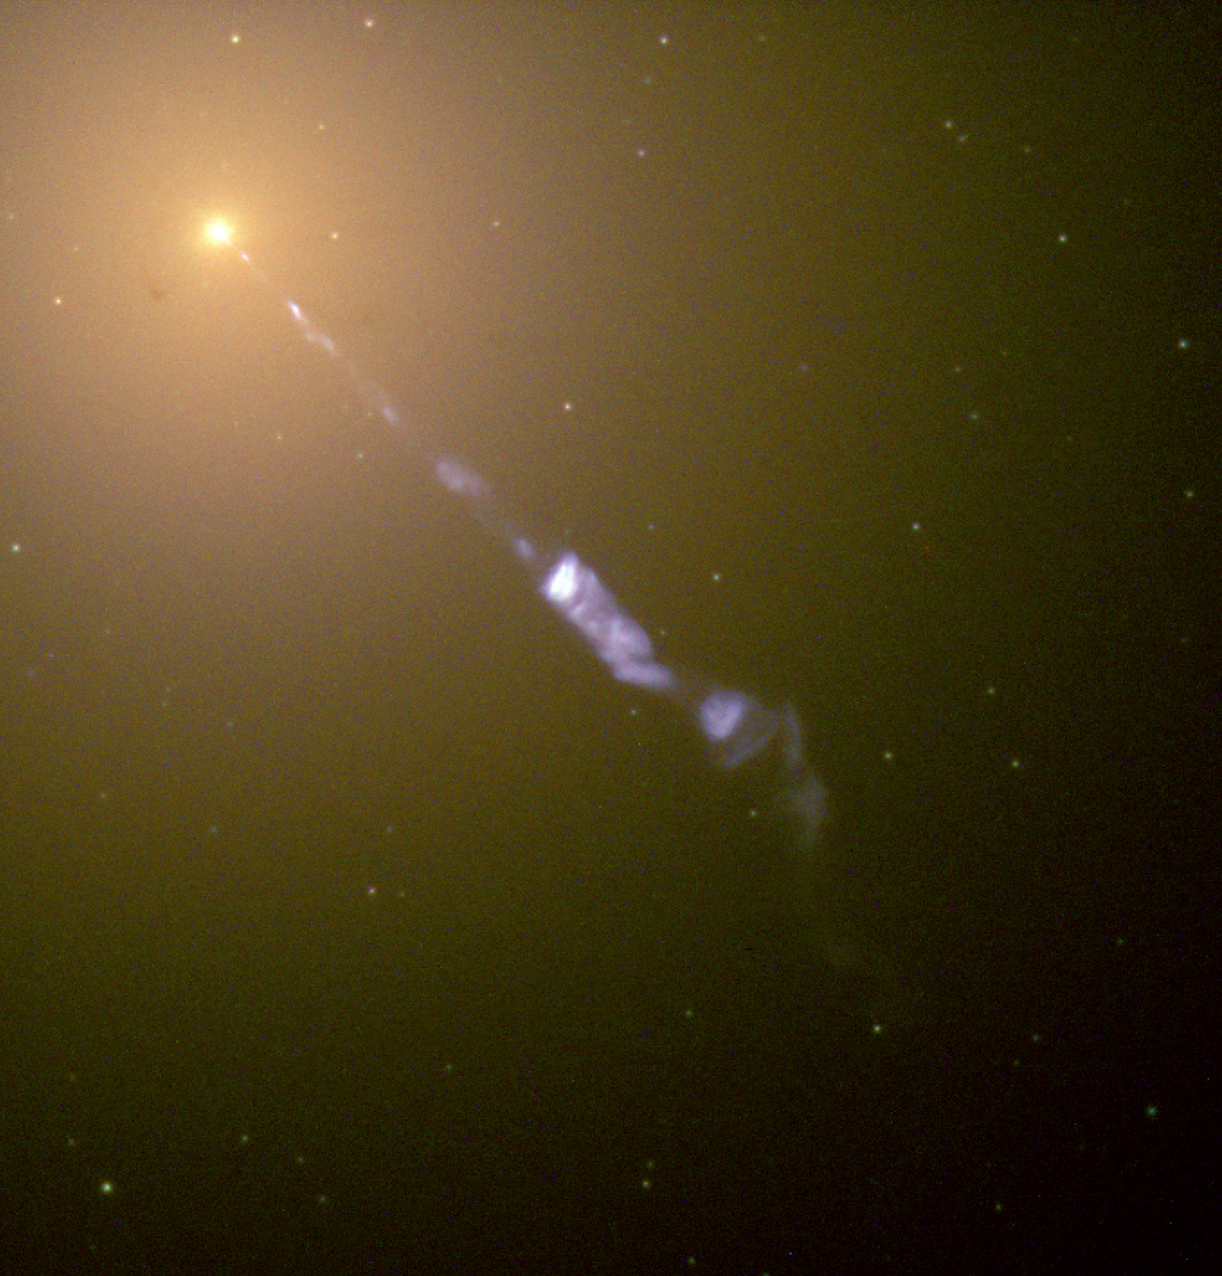
\includegraphics[height=1\unit]{../thesis/images/m87.jpg}\\[-2\baselineskip]
    \color{white}NASA/STSI
  };

  \node[anchor=west, text width=1\unit, align=right] (atmosphere) at (0.5\unit, 0) {%
    \tiny%
    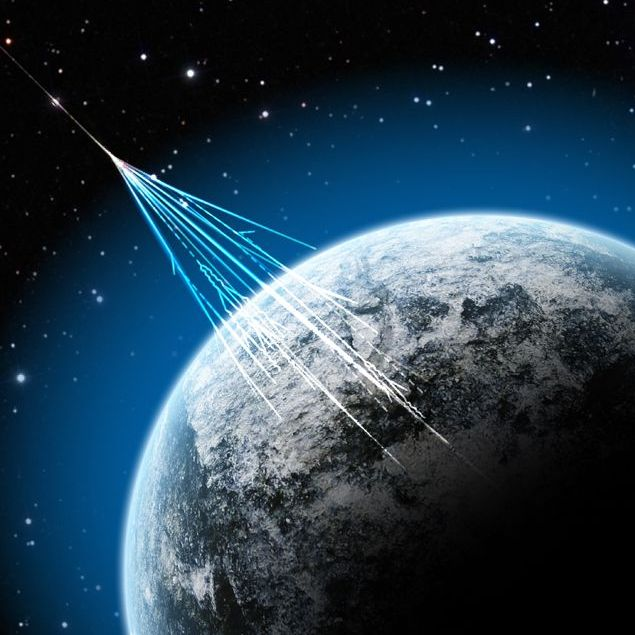
\includegraphics[height=1\unit]{images/airshower.jpg}\\[-2\baselineskip]
    \color{white}NSF/Yang
  };
  \draw[con] (source.east) -- (atmosphere.west);

  \node[anchor=west, text width=\unit, align=center] (telescope) at (2\unit, 0) {
    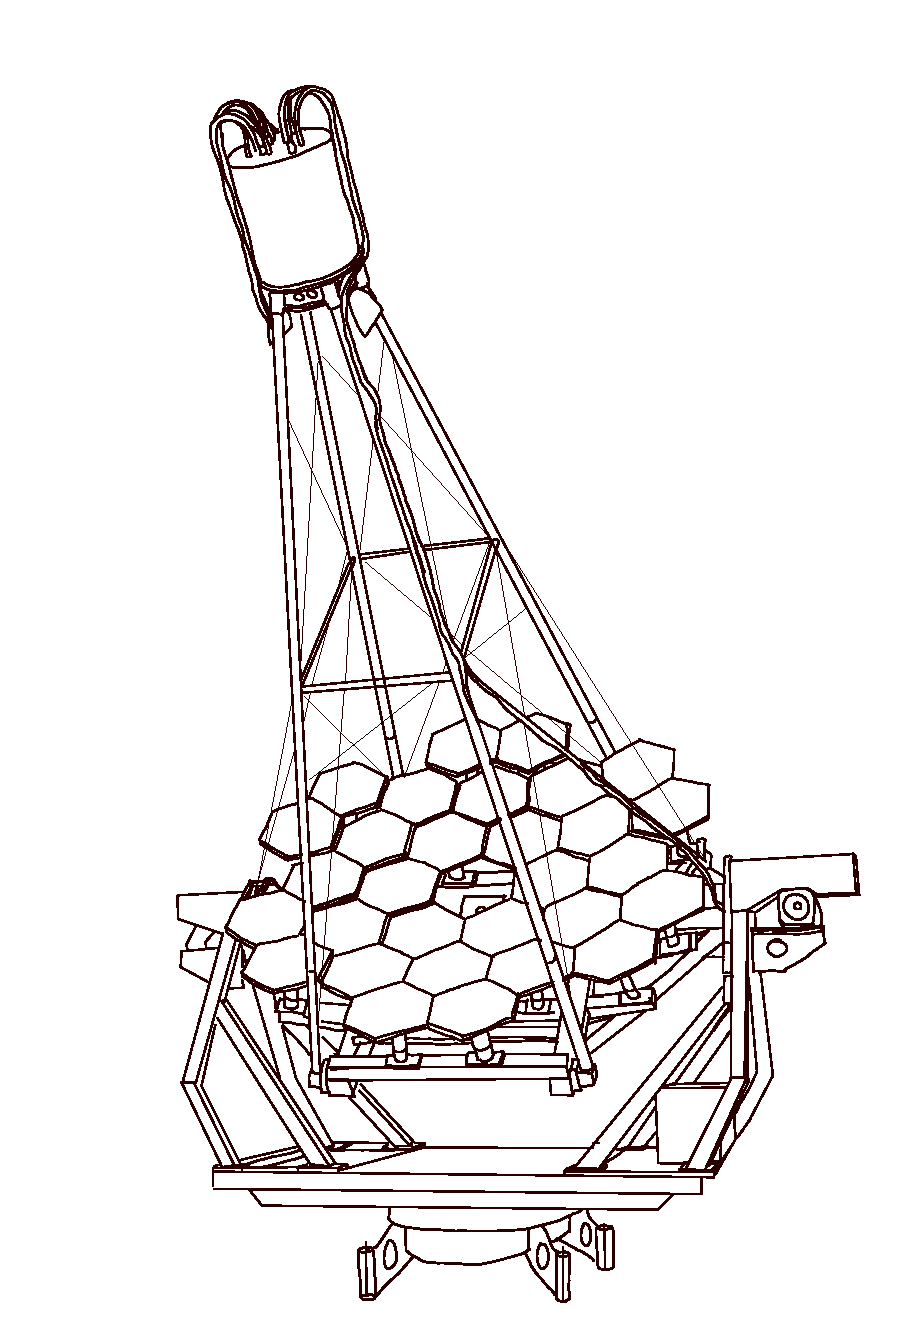
\includegraphics[width=1\unit]{images/fact_sketch.pdf}
  };
  \draw[con] (atmosphere.east) -- (telescope.west);

  \node[anchor=west, text width=\unit, align=center] (corsika) at (0.5\unit, -1.5\unit) {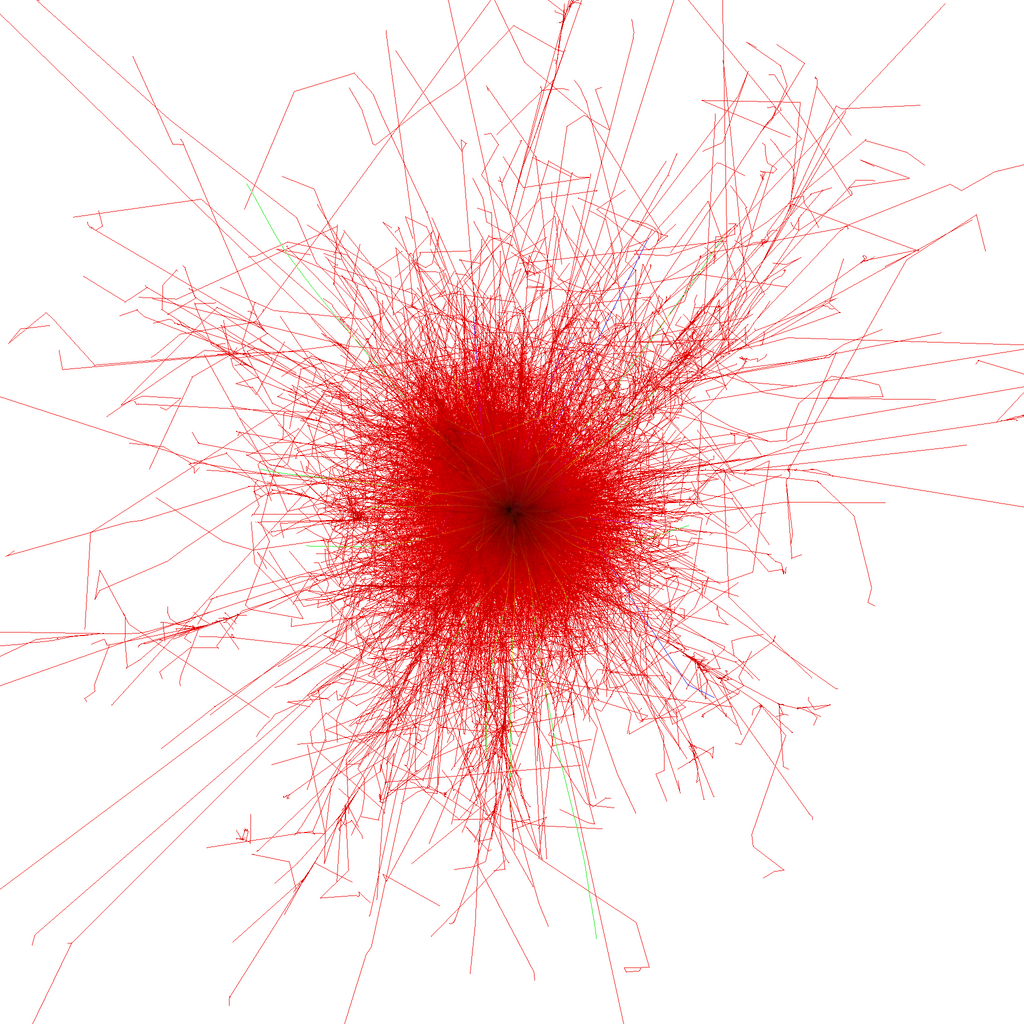
\includegraphics[width=\unit]{images/proton_12_0deg.xy.png}};
  \node[anchor=west, text width=1.1\unit, align=center] at (0.5\unit, -1.75\unit) {\huge\color{black} CORSIKA};

  \node[anchor=west, text width=\unit, align=center] (ceres) at (2\unit, -1.5\unit) {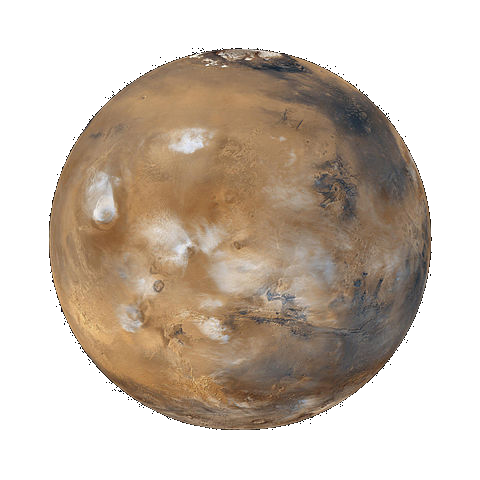
\includegraphics[width=\unit]{images/mars_trim.png}};
  \node[anchor=west, text width=\unit, align=center, fill=white, opacity=0.6, text opacity=1] at (2\unit, -1.75\unit) {\huge\color{black} CERES};
  \draw[con] (corsika.east) -- (ceres.west);

  \node[anchor=west, text width=1.5\unit] (preprocessing) at (3.5\unit, -0.75\unit) {
    \Large Vorverarbeitung \\
    \texttt{FACT-Tools} \\
  };
  \node[anchor=west, text width=1.5\unit] (reco) at (5.5\unit, -0.75\unit) {
    \Large Ereignis-\\Rekonstruktion \\
    \texttt{aict-tools}
  };

  \draw[con] (corsika.east) -- (ceres.west);
  \draw[con] (ceres.east) to[out=0, in=220] (preprocessing.west);
  \draw[con] (telescope.east) to[out=0, in=140] (preprocessing.west);
  \draw[con] (preprocessing.east) -- (reco.west);

\end{tikzpicture}
